\section{Metodologia}

Para concluir com êxito o desenvolvimento deste trabalho e consequentemente os 
objetivos propostos, o método utilizado para solução do problema é composto das 
seguintes etapas sequenciais:

    % coleta de documentos;
    % pr´e-processamento;
    % extra¸c˜ao de conhecimento;
    % avalia¸c˜ao e interpreta¸c˜ao dos resultados.


\subsection{Extração de dados}

% A coleta de documentos ´e respons´avel pela recupera¸c˜ao de documentos relevantes ao
% dom´ınio de aplica¸c˜ao
Após identificar um projeto \cite{brasil_escola}, que estimula o estudante a 
treinar a produção de textos do gênero dissertativo-argumentativo, sugerindo 
um tema, avaliando e armazenando os textos enviados, foi necessário criar um 
\textit{crawler} para extrair estes dados. Existem diversas formas de 
implementar um \textit{crawler}, dentre elas, uma muito utilizada é o 
\textit{Scrapy} \cite{scrapy}, utilizado neste trabalho. O uso de um 
\textit{crawler}, permite explorar a estrutura de grafo da \textit{Web} para 
navegar de uma página para outra, identificando as \textit{tags} HTML que 
contém os dados necessários para compilar um \textit{dataset}. A figura 
\ref{figure:metodologia_1} ilustra a etapa em que o \textit{crawler} navega 
entre as páginas HTML, filtra as \textit{tags}, coleta e armazena os dados em 
um \textit{dataset}.

\begin{figure}[H]
\begin{center}
    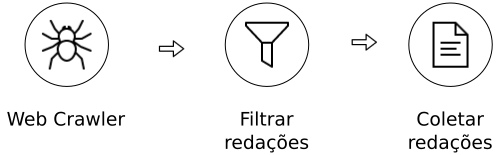
\includegraphics[scale=0.70]{images/metodologia_1.png}
\end{center}
\caption{O \textit{crawler}, navega entre as páginas HTML do banco de redações 
de forma metódica e automatizada indexando textos que posteriormente serão 
filtrados, coletados e armazenados.}
\label{figure:metodologia_1}
\end{figure}

\subsection{Pré-processamento, Indução e Métricas}

Na fase subsequente é utilizada a ferramenta de \textit{Data Mining} 
\cite{orange}. A figura \ref{figure:metodologia_2} ilustra as etapas 
necessárias para pré-processamento, indução e testes dos algoritmos de 
Aprendizado de Máquina. Uma vez gerado o \textit{dataset} ná etapa anterior, no 
primeiro passo os documentos armazenados necessitam de um pré-processamento 
para serem submetidos a indução dos modelos. Devido a sua natureza textual não 
estruturada, cada sentença do texto será separada em \textit{tokens} para 
transformar esses dados não estruturados em um formato estruturado, 
especificamente uma tabela atributo-valor denominada \textit{bag--of--words}. 
Nesta abordagem, palavras pouco significativas como artigos, preposições e 
conjunções que pouco caracterizam os texto podem ser ignoradas com uma ou mais 
listas de \textit{stopwords}. Segundo \cite{matsubara2003pretext}, este passo 
é importante, visto que a representação desses textos tem uma influência 
fundamental no resultado da indução dos algoritmos de Aprendizado de Máquina. 
No segundo passo é necessário definir os parâmetros de inferência de cada 
algoritmo e induzir os modelos classificadores \textit{Adaboost} e 
\textit{Naive Bayes}. O terceiro e último passo, o resultado da inferência dos 
classificadores é avaliada com as principais métricas de análise de 
classificadores citadas na literatura de Aprendizado de Máquina 
(\textit{Acurácia}, Curva ROC e Matriz de confusão). A ferramenta 
\textit{Orange} permite a divisão do \textit{dataset} para a indução e teste, 
bem como, a inferência simultanea de vários classificadores. O resultados das 
métricas de desempenho são plotados para avaliação e comparação dos 
classificadores induzidos. Os passos dois e três são repetidos até que um do 
classificadores apresente resultados relevantes ao estudo.

\begin{figure}[H]
\begin{center}
    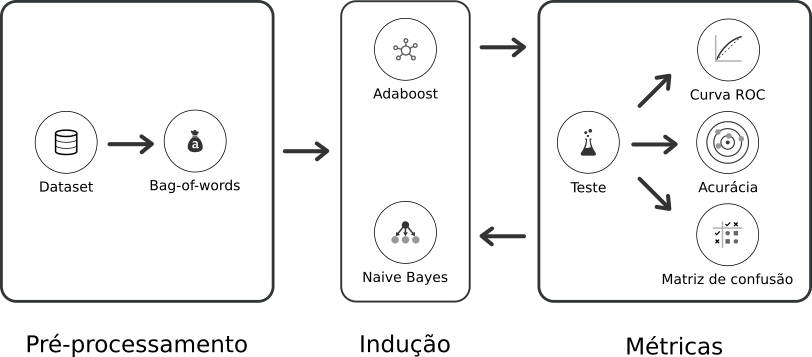
\includegraphics[scale=0.70]{images/metodologia_2.png}
\end{center}
\caption{Os textos são submetidos aos algoritmos de normalização e posteriormente estruturados e armazenados no padrão JSON.}
\label{figure:metodologia_2}
\end{figure}

% Na terceira etapa ilustrada pela Figura ~\ref{figure:metodologia_3} será utilizada a ferramenta de mineração de dados \textit{Orange} ~\cite{JMLR:demsar13a}. Será necessário realizar estudo e análise para obter o conhecimento necessário para desenvolvimento de um fluxo de trabalho, seleção e treinamento dos modelos classificadores, concluindo todos os objetivos propostos nesta etapa.

% \begin{figure}[H]
% \begin{center}
%     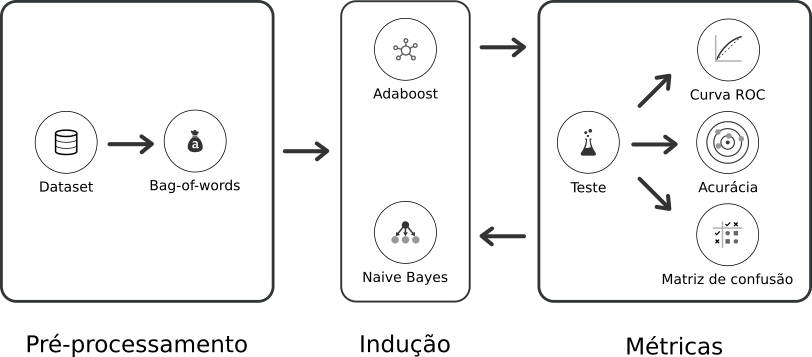
\includegraphics[scale=0.75]{images/metodologia_3.png}
% \end{center}
% \caption{O \textit{corpus} será utilizado em um fluxo de trabalho da ferramenta \textit{Orange} para treinar os modelos classificadores.}
% \label{figure:metodologia_3}
% \end{figure}

% A quarta e última etapa é ilustrada pela Figura ~\ref{figure:metodologia_4}, onde o classificador previamente ajustado e treinado será submetido aos testes de Acurácia, Sensitividade, Precisão, Especificidade, Curva ROC e Matriz de Confusão. Os resultados serão representados graficamente e comparados para analisar o desempenho do classificador.
% \begin{figure}[H]
% \begin{center}
%     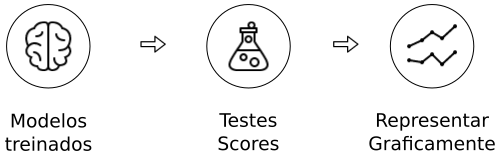
\includegraphics[scale=0.75]{images/metodologia_4.png}
% \end{center}
% \caption{O classificador ajustado e treinado será submetido a testes, e os resultados comparados graficamente com o objetivo de analisar o desempenho do classificador induzido.}
% \label{figure:metodologia_4}
% \end{figure}
